
Fitting and plotting various trends

\begin{lstlisting}
# time plot of U.S. GNP and various fitted trends
par(mfrow=c(2,2))
par(oma=c(0,2,4,2))

# global quadratic trend
plot(x=1947.25+gnp.t,y=gnp.v,type="b",ylim=c(200,800),xlab="time",ylab="U.S. GNP",main="Global quadratic trend",col="green4")
lines(1947.25+gnp.t,predict(object=gqt.lm),col="blue")
legend(x="topleft",legend=c("actual values","estimated global trend"),col=c("green4","blue","red"),lty=c(1,1),pch=c(1,-1))

# global cubic trend
plot(x=1947.25+gnp.t,y=gnp.v,type="b",ylim=c(200,800),xlab="time",ylab="U.S. GNP",main="Global cubic trend",col="green4")
lines(1947.25+gnp.t,predict(object=gct.lm),col="blue")

# global multiplicative exponential trend
plot(x=1947.25+gnp.t,y=gnp.v,type="b",ylim=c(200,800),xlab="time",ylab="U.S. GNP",main="Global multiplicative exponential trend",col="green4")
lines(1947.25+gnp.t,exp(predict(object=gmet.lm)),col="blue")

# global additive exponential trend
plot(x=1947.25+gnp.t,y=gnp.v,type="b",ylim=c(200,800),xlab="time",ylab="U.S. GNP",main="Global additive exponential trend",col="green4")
lines(1947.25+gnp.t,predict(object=gaet.nls),col="blue")

mtext(text="Time plots of U.S. GNP and fitted trends",side=3,line=0,outer=T)
\end{lstlisting}

\begin{figure}[H]
\centering
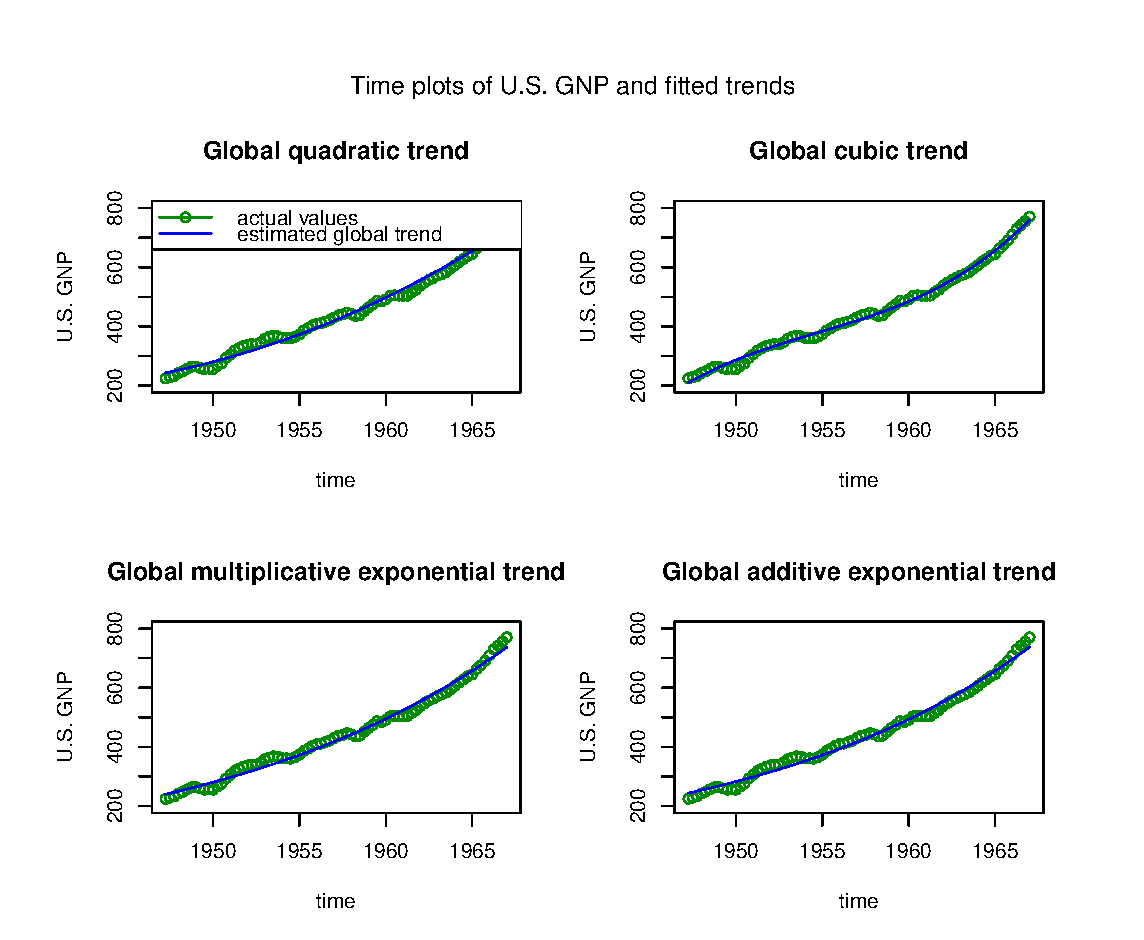
\includegraphics[width=0.8\textwidth]{plots/Rplot1.pdf}
\caption{Various Fits}
\end{figure}

\subsection{Analysis of Precipitation and Temperature Data in Zurich}

We begin our analysis by looking at the raw series and a deseasonalized series for the precipitation data:

\begin{lstlisting}
# define variables
  sf=1
  raw.data.ex.season <- deseason(raw.data)
  raw.data.ex.trend.KS <- detrend(raw.data,ma=F,sf)
  raw.data.ex.trend.KS.ex.season <- deseason(raw.data.ex.trend.KS$detrended.series)
  
# define axis labels
  acf.x.lab <- expression(paste("lag ",tau,sep=""))
  acf.y.lab <- expression(paste("acf(",tau,")",sep=""))

# time plot and correlogram of deseasonalized data 
  par(mfrow=c(2,2))
  par(oma=c(0,2,4,2))
  plot(x=raw.data,type="b",xlab="Time",ylab=ylabel,main="Raw series",col=line.color)
  plot(x=raw.data.ex.season$deseasoned.series,type="b",xlab="Time",ylab=ylabel,main="Deseasonalized series",col=line.color)
  acf(x=raw.data,xlab=acf.x.lab,ylab=acf.y.lab,main="")
  acf(x=raw.data.ex.season$deseasoned.series,xlab=acf.x.lab,ylab=acf.y.lab,main="")
  mtext(text=title.text,side=3,line=0,outer=T)
\end{lstlisting}

\begin{figure}[H]
\centering
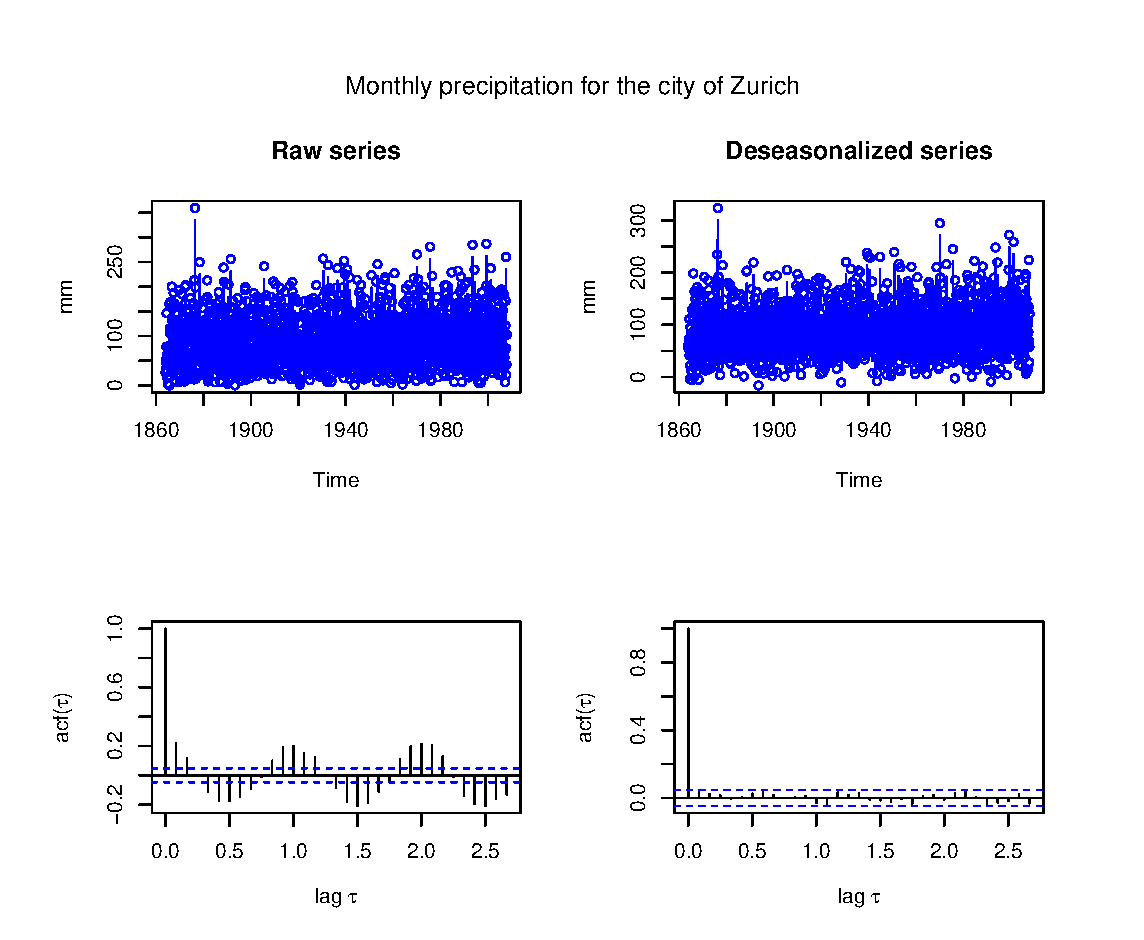
\includegraphics[width=0.8\textwidth]{plots/ZHP1.pdf}
\caption{Precipitation}
\end{figure}

The correlogram for the raw series shows that there is a lot of significant correlation at almost all lags and there is a clear seasonal pattern to it. Whereas the deseasonalized correlogram makes the series appear stationary. \\

To confirm that there is a seasonal effect we look at this effect on its own: 

\begin{lstlisting}
# plot of seasonal effects [ZHP2]
  par(mfrow=c(1,1))
  par(oma=c(0,2,4,2))
  plot(raw.data.ex.season$season.effects,type="b",col=line.color,xlab="Month",ylab="Effect",main="Seasonal effects")
\end{lstlisting}


\begin{figure}[H]
\centering
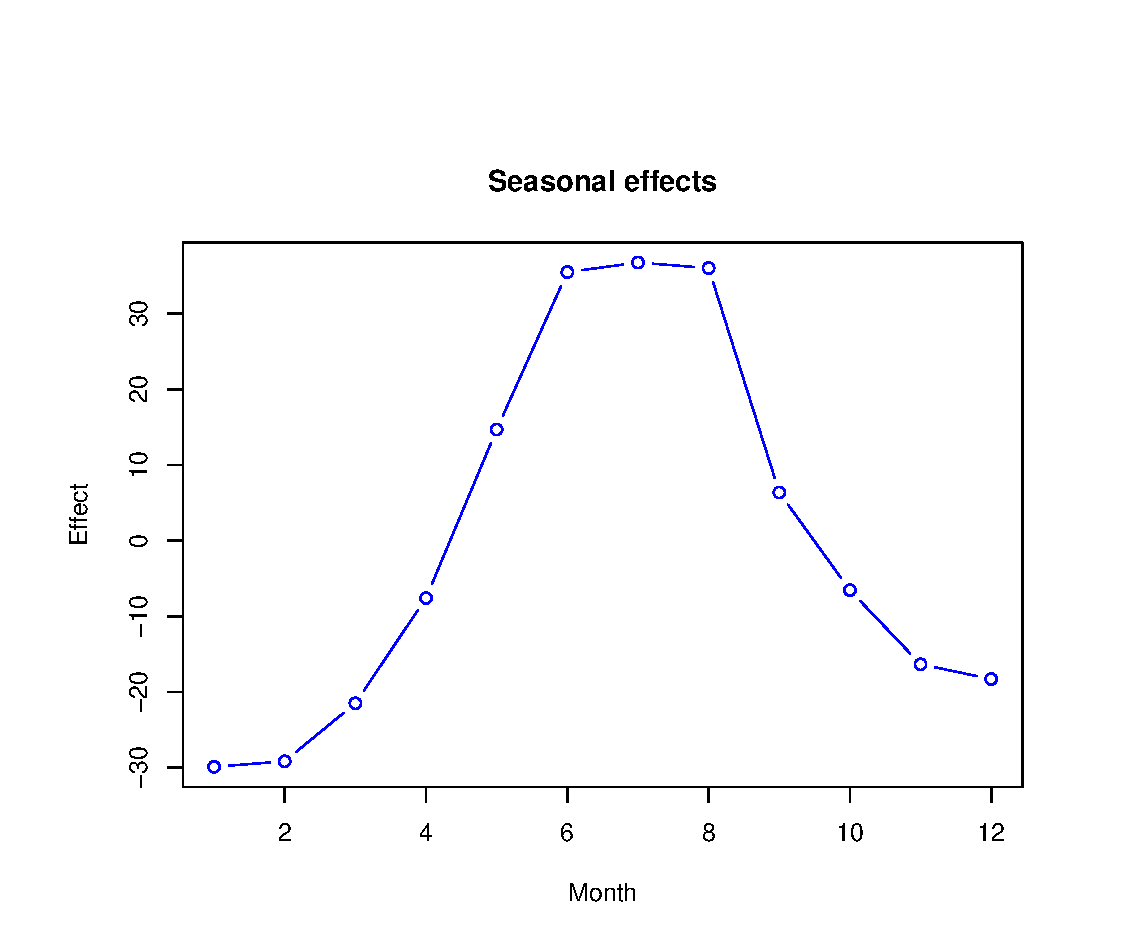
\includegraphics[width=0.6\textwidth]{plots/ZHP2.pdf}
\caption{Seasonal effects}
\end{figure}

When we look at the temperature data, we can observe that there is a linear trend in the raw series. But as the middle graph shows differencing alone does not make the series stationary, we again need to deseasonalize it.

\begin{lstlisting}
# time plots and correlograms of deseasonalized KS-detrended data
  par(mfrow=c(2,3))
  par(oma=c(0,2,4,2))
  plot(x=raw.data,type="b",xlab="time",ylab=ylabel,main="raw series",col=line.color)
  lines(x=as.numeric(time(raw.data.ex.trend.KS$trend)),y=as.numeric(raw.data.ex.trend.KS$trend),col="red")
  plot(x=raw.data.ex.trend.KS$detrended.series,type="b",xlab="Time",ylab=ylabel,main="KS-detrended series",col=line.color)
  plot(x=raw.data.ex.trend.KS.ex.season$deseasoned.series,type="b",xlab="time",ylab=ylabel,main="deseasonalized KS-detrended series",col=line.color)
  acf(x=raw.data,xlab=acf.x.lab,ylab=acf.y.lab,main="")
  acf(x=raw.data.ex.trend.KS$detrended.series,xlab=acf.x.lab,ylab=acf.y.lab,main="")
  acf(x=raw.data.ex.trend.KS.ex.season$deseasoned.series,xlab=acf.x.lab,ylab=acf.y.lab,main="")
  mtext(text=paste(title.text," (KS-detrended)",sep=""),side=3,line=0,outer=T)
\end{lstlisting}

\begin{figure}[H]
\centering
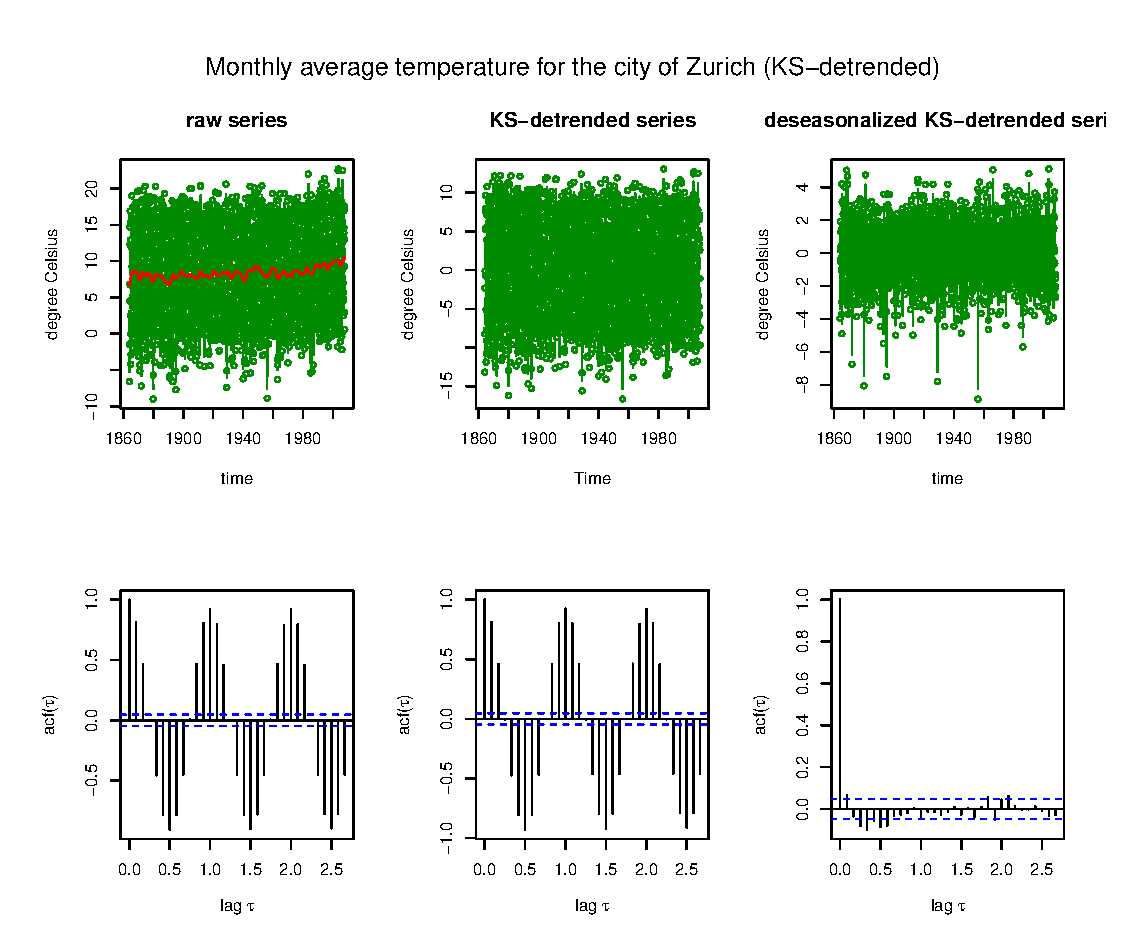
\includegraphics[width=0.8\textwidth]{plots/ZHP4.pdf}
\caption{Temperature}
\end{figure}

\subsection{Unemployment Data}


\begin{figure}[H]
\centering
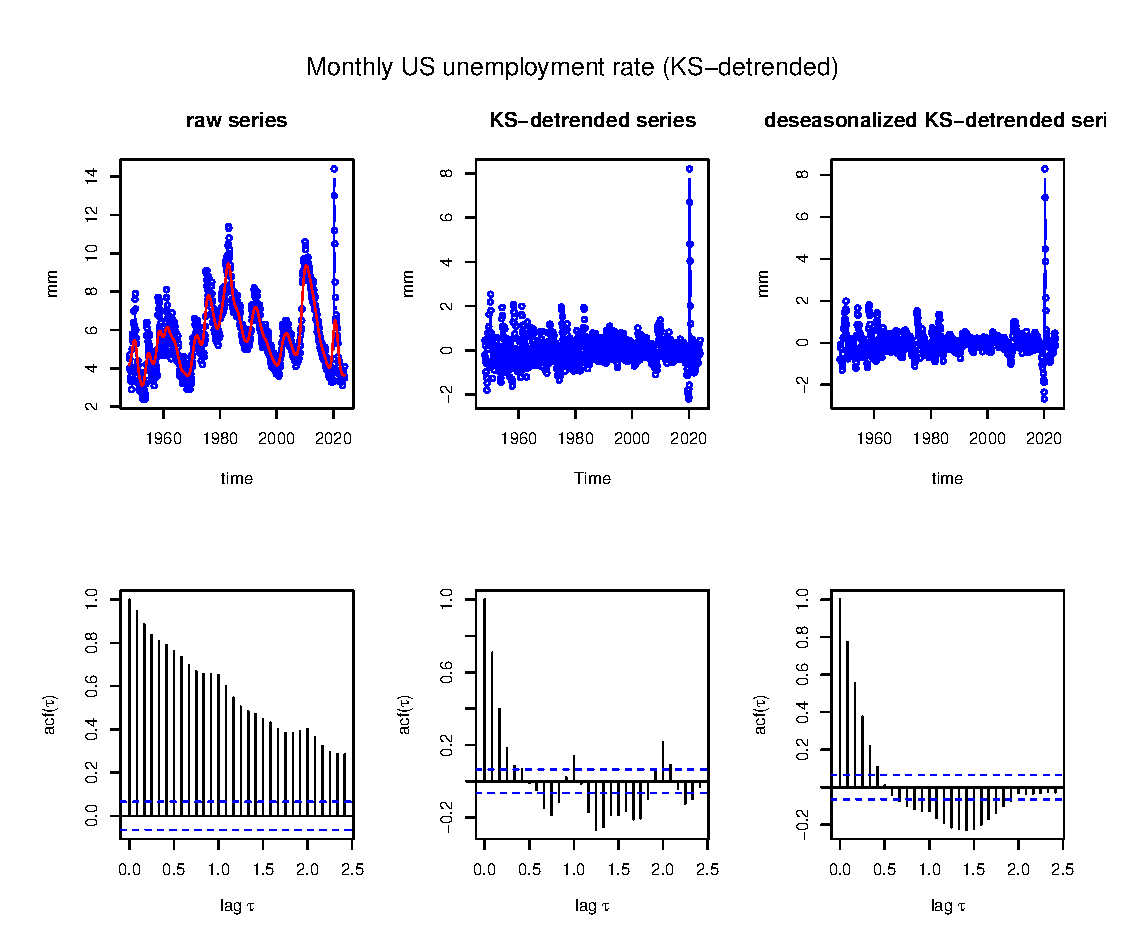
\includegraphics[width=0.8\textwidth]{plots/UEMP.pdf}
\caption{Unemployment}
\end{figure}

We see looking at the raw data, the trend line and the correlogram, that there is significant correlation at all lags. After detrending the correlogram shows that the trend is somewhat dissappeared, but there is still seasonality.

\subsection{Stock data}

\begin{lstlisting}
stock <- read.csv('/Users/michaelsigg/Desktop/Master/FS24/Time Series Analysis/Exc. 3/NVDA.csv', sep=',') # https://finance.yahoo.com/quote/NVDA/history?period1=916963200&period2=1709856000&interval=1d&filter=history&frequency=1d&includeAdjustedClose=true
stock$Date <- as.Date(stock$Date, "%Y-%m-%d")
stock$LogClose = log(stock$Close)

stock$DeltaClose = c(NA, diff(stock$Close))

stock$LogClose = log(stock$Close)
stock$DeltaLogClose = c(NA, diff(stock$LogClose))

par(mfrow=c(2,2))
par(oma=c(0,2,4,2))
plot(stock$Date, stock$Close, type = 'l', xlab = "Time", ylab = "Close Price", main = 'Close Price')
plot(stock$Date, stock$LogClose, type = 'l', xlab = "Time", ylab = "Log Close Price", main = 'Log(Close Price)')
plot(stock$Date, stock$DeltaClose, type = 'l', xlab = "Time", ylab = "Delta Close Price", main = 'Differenced Close Price')
plot(stock$Date, stock$DeltaLogClose, type = 'l', xlab = "Time", ylab = "Delta Log Close Price", main = 'Differenced Log(Close Price)')
mtext(text="NVIDIA historical price charts",side=3,line=0,outer=T)
\end{lstlisting}

\begin{figure}[H]
\centering
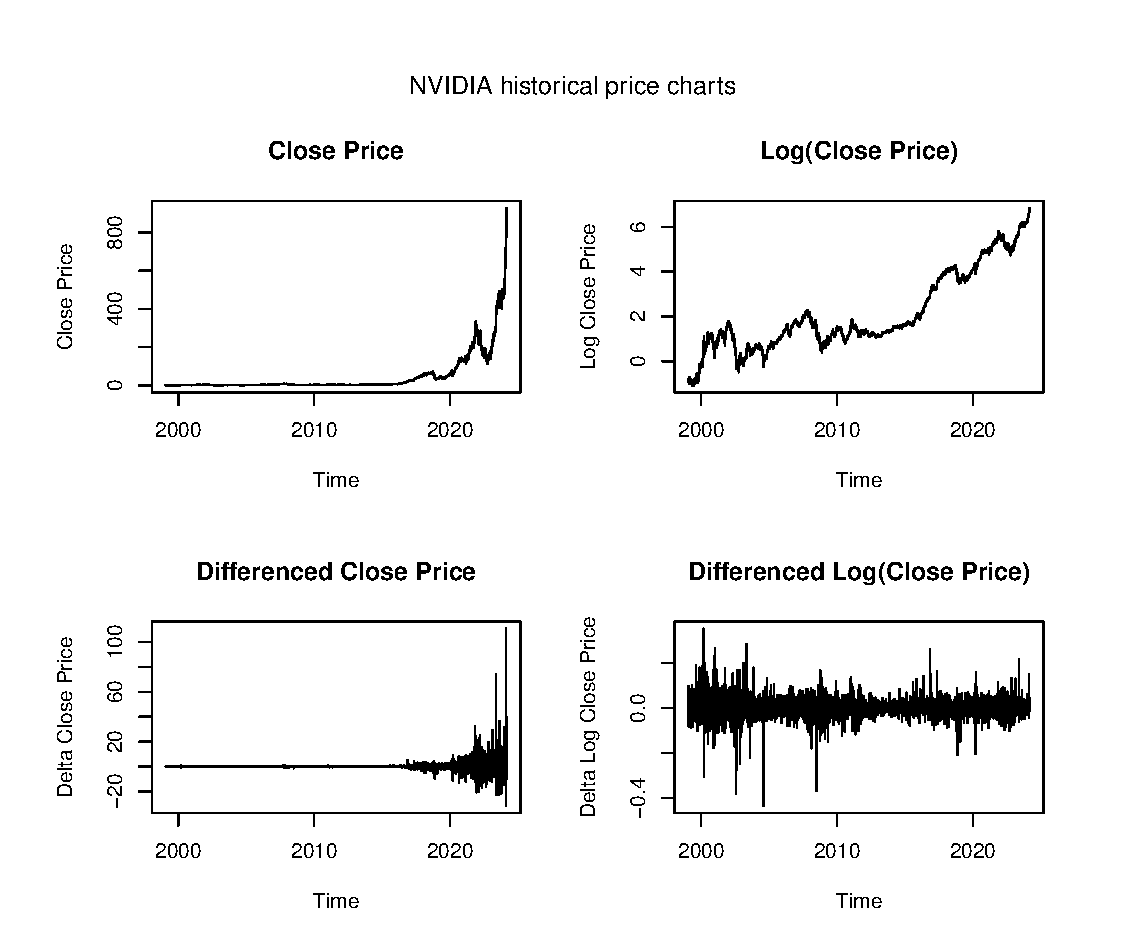
\includegraphics[width=0.8\textwidth]{plots/NVD.pdf}
\caption{NVIDIA Price Charts}
\end{figure}

Already at first look, it is clear that differencing the data is not enough to make it stationary. Lets look at the autocorrelation and partial autocorrelation function:

\begin{lstlisting}
stock.acf <- acf(na.omit(stock$DeltaClose), lag.max = 100, main = "Delta Close Price")
stock.pacf <- pacf(na.omit(stock$DeltaClose), lag.max = 100, main = "Delta Close Price")

logstock.acf <- acf(na.omit(stock$DeltaLogClose), lag.max = 100, main = "Delta Log Close Price")
logstock.pacf <- pacf(na.omit(stock$DeltaLogClose), lag.max = 100, main = "Delta Log Close Price")
\end{lstlisting}

\begin{figure}[H]
\centering
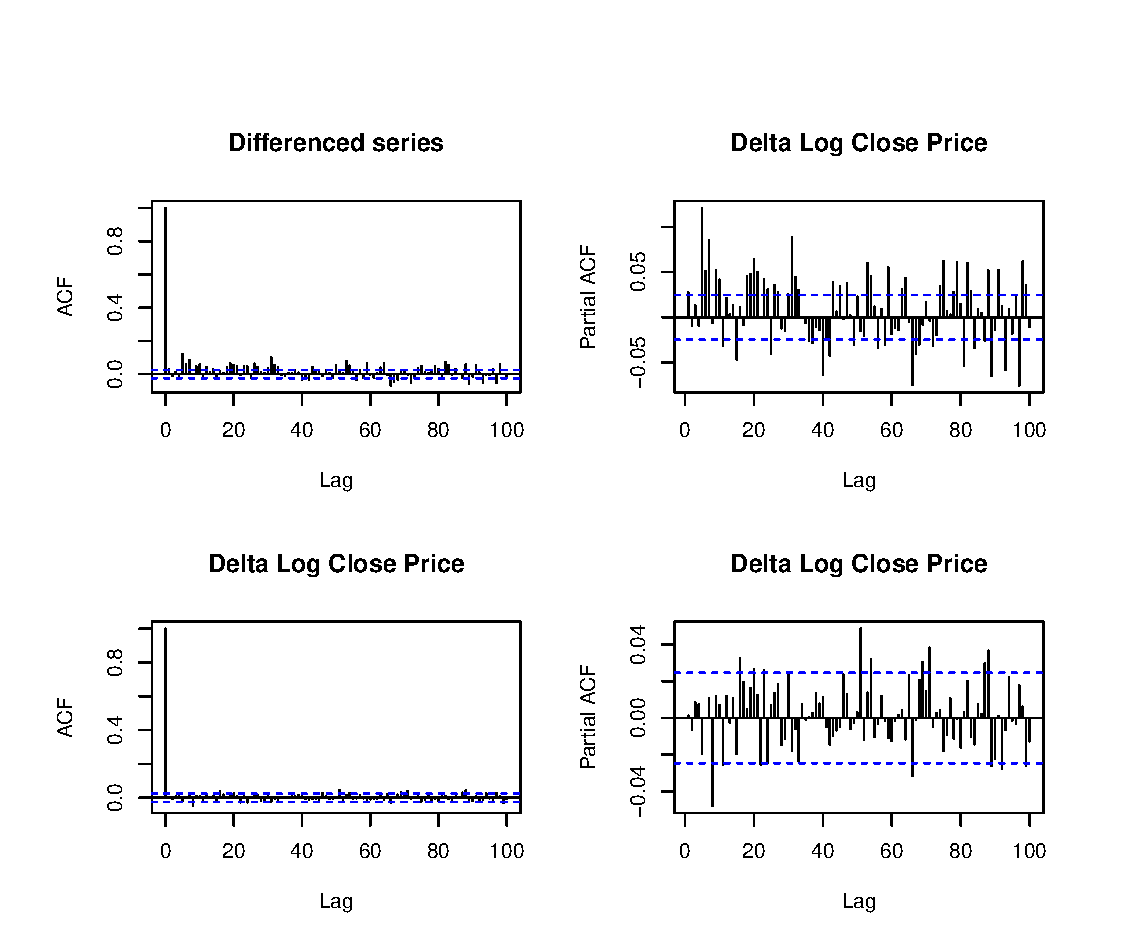
\includegraphics[width=0.8\textwidth]{plots/NVD2.pdf}
\caption{NVIDIA Correlograms}
\end{figure}

We see here that both the acf and the pacf for the differenced data indicates non-stationarity. Taking the log addresses this issue. (Note that the lags that still have significant correlation are expected to appear just by chance. As we have a 95\% CI, out of 100 lags we'd expect around 5 to have significant correlation just by chance). 

\begin{lstlisting}
fit.diff <- arima(stock$DeltaClose, c(0,0,0))
fit.diff
tsdiag(fit.diff)

\end{lstlisting}

\begin{figure}[H]
\centering
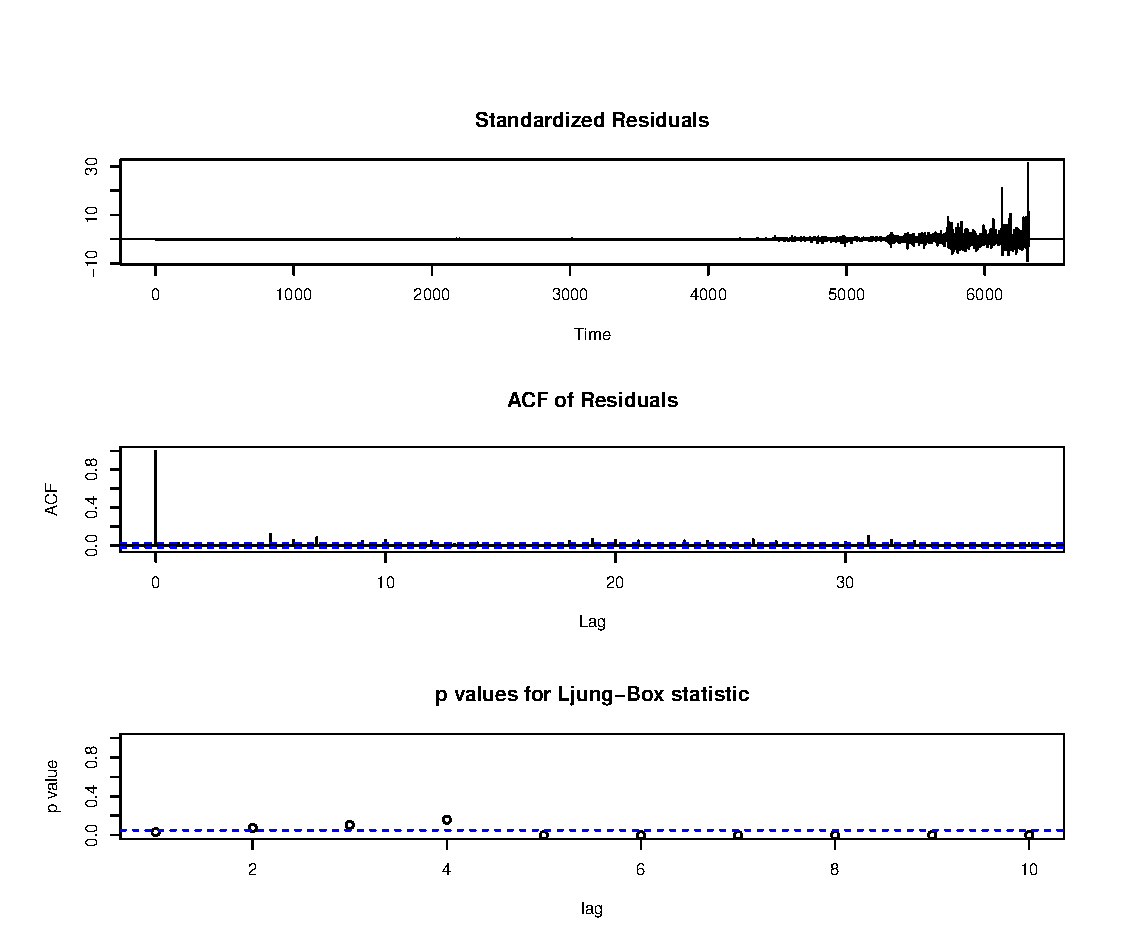
\includegraphics[width=0.8\textwidth]{plots/NVD3.pdf}
\caption{Differenced Closing Price}
\end{figure}

This shows that when we fit an ARMA(0,0,0) model (i.e., a white noise process) the residuals still shows significant correlation at various lags. And the Ljung-Box Statistic confirms that we can reject the null hypothesis of no autocorrelation for several lag intervals, it confirms that the residuals are not white noise. 

\begin{lstlisting}
fit.diff.log <- arima(stock$DeltaLogClose, c(0,0,0))
fit.diff.log
tsdiag(fit.diff.log)
\end{lstlisting}

\begin{figure}[H]
\centering
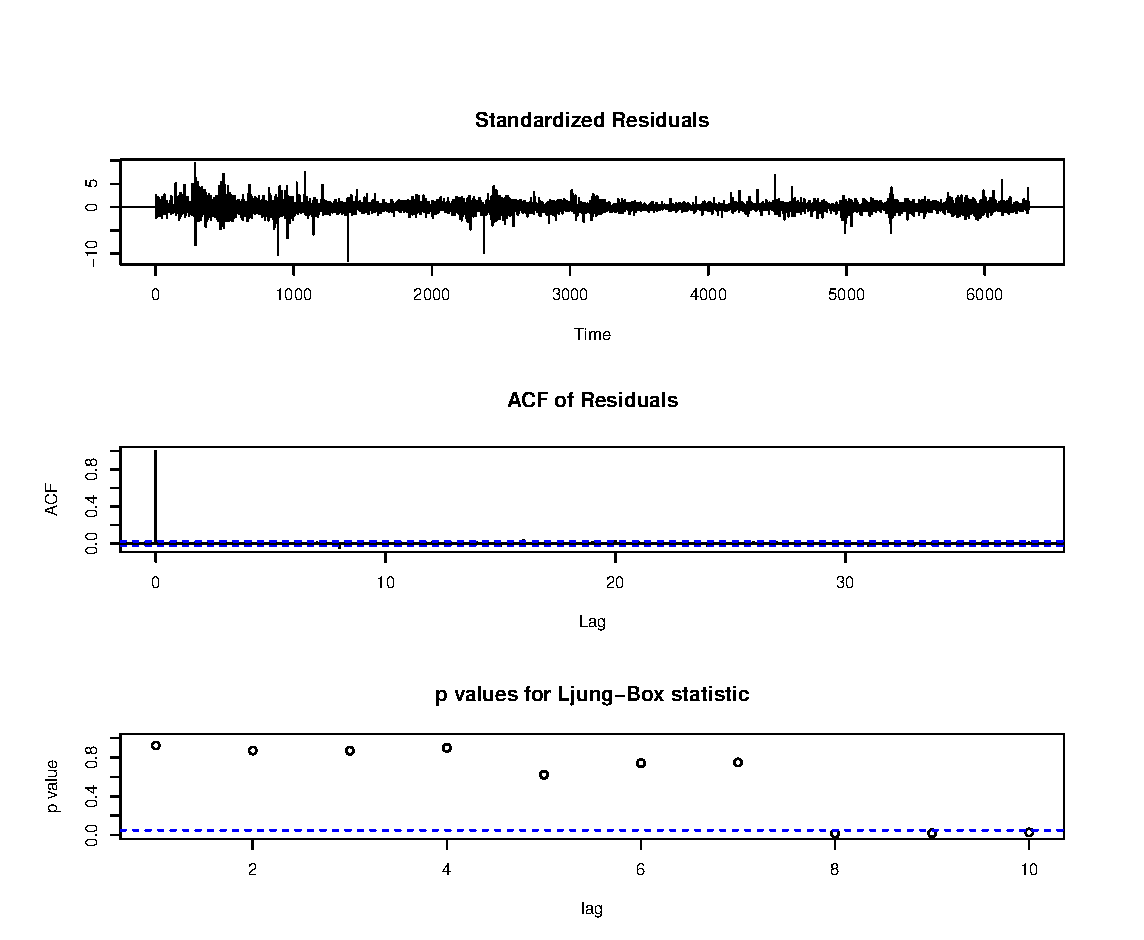
\includegraphics[width=0.8\textwidth]{plots/NVD4.pdf}
\caption{Differenced Log Closing Price }
\end{figure}

 When we fit the same ARMA(0,0,0) model to the log data, we can see that the residuals show no signs of autocorrelation and we can not reject the null hypothesis of the Ljung-Box Test, that the residuals are not white noise. 

\subsection{U.S. Production Index}


We start by reading in the data and setting some global variables:\\



\begin{lstlisting}
# user in put
acf.lag.max <- 36 # max lag for ac.f./pac.f.
raw.SARIMA.spec <- list(p=1,d=1,q=1,P=2,D=1,Q=1,freq=12) # SARIMA model for raw series
log.SARIMA.spec <- list(p=1,d=1,q=1,P=2,D=1,Q=1,freq=12) # SARIMA model for log series
forecast.horizon <- 12 # specifications for forecasting: horizon
forecast.level <- 95 # specifications for forecasting: confidence level for prediction intervals


# load 'class.RData'
load("/Users/michaelsigg/Desktop/Master/FS24/Time Series Analysis/Exc. 7/class.rdata")

# definition of delimiters for output
delimiter.stars <- paste("\n",paste(rep("*",80),sep="",collapse=""),"\n",sep="")
delimiter.hyphen <- paste(paste(rep("-",80),sep="",collapse=""),"\n",sep="")


# define time series
ts.data.raw <- fed.prod
ts.data.1stdiff <- diff(ts.data.raw)
ts.data.log <- log(ts.data.raw)
ts.data.log.1stdiff <- diff(ts.data.log,1)
\end{lstlisting}

We first plot the raw series: \\

\begin{lstlisting}
# plot time series and associated ac.f and pac.f and (raw series)
layout(matrix(c(1,1,2,2,3,4,5,6),nr=2,byrow=TRUE))
par(oma=c(0,2,4,2))
plot(x=ts.data.raw,type="b",xlab="time",ylab="",main="raw series",col="green4",font.main=1,cex.main=1) 
plot(x=ts.data.1stdiff,type="b",xlab="time",ylab="",main="first differences of raw series",col="green4",font.main=1,cex.main=1)
acf(x=ts.data.raw,lag.max=acf.lag.max,type="correlation",xlab="lag",ylab="ac.f.",main="")
title(main="sample ac.f.",font.main=1,cex.main=1)
acf(x=ts.data.raw,lag.max=acf.lag.max,type="partial",xlab="lag",ylab="pac.f.",main="") 
title(main="sample pac.f.",font.main=1,cex.main=1) 
acf(x=ts.data.1stdiff,lag.max=acf.lag.max,type="correlation",xlab="lag",ylab="ac.f.",main="")
title(main="sample ac.f.",font.main=1,cex.main=1)
acf(x=ts.data.1stdiff,lag.max=acf.lag.max,type="partial",xlab="lag",ylab="pac.f.",main="")
title(main="sample pac.f.",font.main=1,cex.main=1)
mtext(text="Exercise 7.1: U.S. Production Index (raw series)",side=3,line=0,outer=T,font=2,cex=1)
\end{lstlisting}

\begin{figure}[H]
\centering
\includegraphics[width=0.8\textwidth]{plots/UsProdRaw.pdf}
\caption{U.S. Production Index Raw Series}
\end{figure}
The raw series is clearly non-stationary due to its upward trend. To address this, we apply a log transformation:

\begin{figure}[H]
\centering
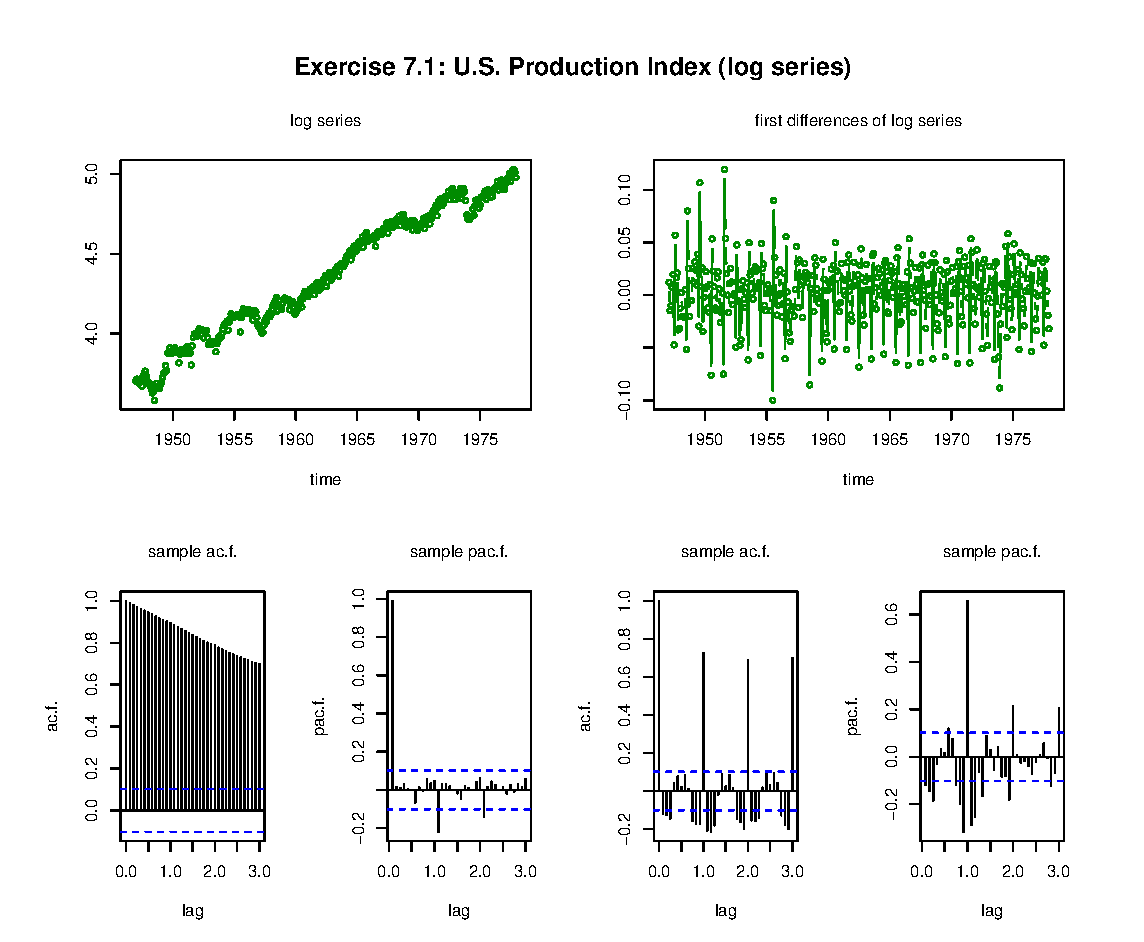
\includegraphics[width=0.8\textwidth]{plots/UsProdRawLog.pdf}
\caption{U.S. Production Index Log Series}
\end{figure}

The log transformation, followed by differencing, makes the series more stationary. The ac.f. and pac.f. plots indicate some remaining autocorrelation, but the situation is improved.\\

Next, we estimate a SARIMA model on the raw series and examine the diagnostics: \\


\begin{lstlisting}
# estimate SARIMA model (raw series)
ts.data.raw.fit <- arima(x=ts.data.raw,order=c(raw.SARIMA.spec$p,raw.SARIMA.spec$d,raw.SARIMA.spec$q),seasonal=list(order=c(raw.SARIMA.spec$P,raw.SARIMA.spec$D,raw.SARIMA.spec$Q),period=raw.SARIMA.spec$freq))


# diagnostic plots (raw series)
layout(mat=matrix(c(1,1,1,2,3,4),nr=2,byrow=TRUE),heights=c(1,1))
par(oma=c(0,2,12,2))
plot(x=ts.data.raw.fit$residuals,type="b",xlab="time",ylab="",main="standardized residuals",col="green4",font.main=1,cex.main=1)
acf(x=ts.data.raw.fit$residuals,lag.max=acf.lag.max,type="correlation",xlab="lag",ylab="ac.f.",main="")
title(main="sample ac.f. of standardized residuals",font.main=1,cex.main=1)
acf(x=ts.data.raw.fit$residuals,lag.max=acf.lag.max,type="partial",xlab="lag",ylab="ac.f.",main="")
title(main="sample pac.f. of standardized residuals",font.main=1,cex.main=1)
Ljung.Box.p.value <- NULL
for (k in 1:acf.lag.max)
  Ljung.Box.p.value <- c(Ljung.Box.p.value, Box.test(x=ts.data.raw.fit$residuals,lag=k,type="Ljung-Box")$p.value)
plot(x=(1:acf.lag.max)/12,y=Ljung.Box.p.value,ylim=c(0,1),xlab="lag",ylab="p-value",main="p-values for Ljung-Box statistics",col="green4",font.main=1,cex.main=1)
lines(x=c(-5,acf.lag.max+5),y=0.05*c(1,1),col="red",lty=2)
mtext(text="Exercise 7.1: U.S. Production Index - raw series - diagnostic plots",side=3,line=6,outer=T,font=2,cex=1)
mtext(paste("model: ",trim(capture.output(ts.data.raw.fit)[2]),sep=""),side=3,line=1,outer=T,at=0.5)
\end{lstlisting}

\begin{figure}[H]
\centering
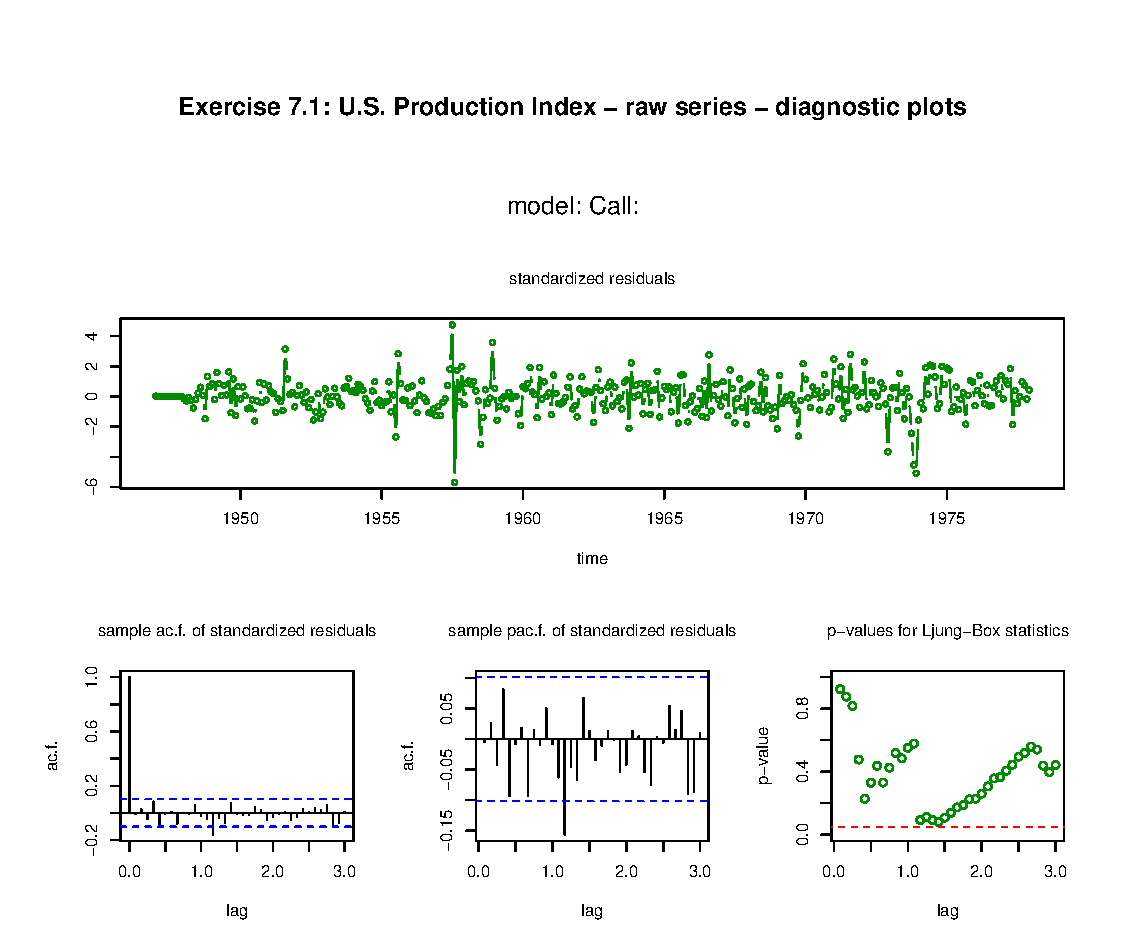
\includegraphics[width=0.8\textwidth]{plots/UsProdRawDiag.pdf}
\caption{U.S. Production Index Raw Diagnostics}
\end{figure}
The standardized residuals should ideally show no obvious pattern. However, for the raw series, some periods have larger residuals, indicating potential heteroscedasticity. The ac.f. shows significant autocorrelations at multiple lags, suggesting the model hasn't fully captured the data's dependencies. Similarly, the pac.f. indicates remaining structure in the residuals. The Ljung-Box statistics show p-values below the threshold, indicating significant autocorrelations, suggesting that the model may not be adequate.\\

\begin{figure}[H]
\centering
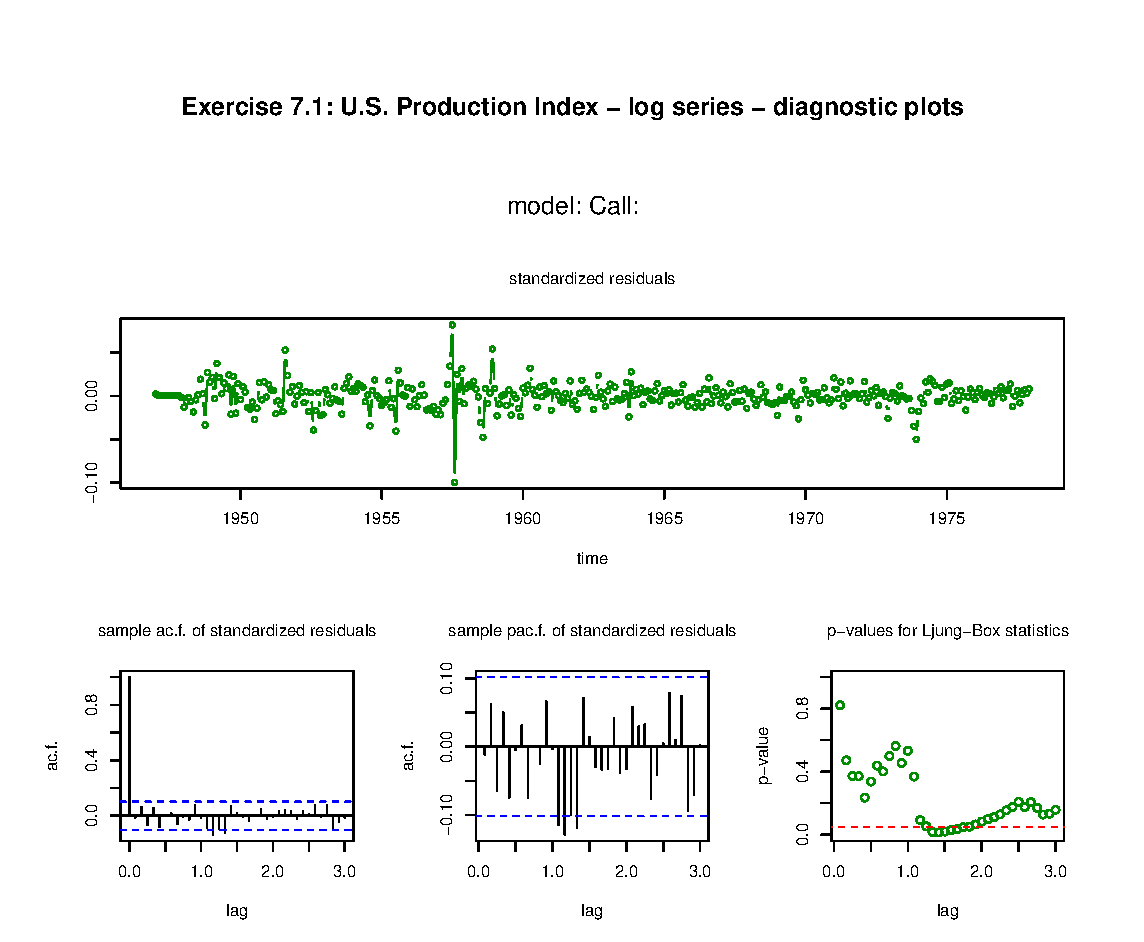
\includegraphics[width=0.8\textwidth]{plots/UsProdLogDiag.pdf}
\caption{U.S. Production Index Log Diagnostics}
\end{figure}

For the log-transformed series, the residuals are more stable, indicating that the log transformation may have helped stabilize the variance. The ac.f. and pac.f. show fewer significant autocorrelations, suggesting a better model fit. The Ljung-Box statistics also indicate fewer autocorrelations, suggesting the residuals are closer to white noise.\\

We now make forecasts on both series using our estimated SARIMA model and exponential smoothing:\\

\begin{lstlisting}
# forecast with exponential smoothing
ts.data.raw.ets <- ets(y=ts.data.raw)
ts.data.log.ets <- ets(y=ts.data.log)
ts.data.raw.ets.pred <- forecast(object=ts.data.raw.ets,h=forecast.horizon,level=forecast.level)
ts.data.log.ets.pred <- forecast(object=ts.data.log.ets,h=forecast.horizon,level=forecast.level)



# forecast with SARIMA
ts.data.raw.sarima.pred <- forecast(object=ts.data.raw.fit,h=forecast.horizon,level=forecast.level)
ts.data.log.sarima.pred <- forecast(object=ts.data.log.fit,h=forecast.horizon,level=forecast.level)



# plot point forecasts and forecast intervals (raw series)
layout(matrix(c(1,1,2,3,3,4),nr=2,byrow=T))
par(oma=c(0,2,4,2))
plot(x=ts.data.raw.ets.pred,include=12*10,shaded=T,shadecols="pink1",main="",col="blue",fcol="red",type="b",xlab="time")
title(main="Forecast method: SARIMA",font.main=1,cex.main=1)
qqnorm(y=ts.data.raw.ets.pred$residuals,main="",col="green4")
qqline(y=ts.data.raw.ets.pred$residuals,col="black")
title(main="Normal Q-Q plot for residuals",font.main=1,cex.main=1)
plot(x=ts.data.raw.sarima.pred,include=12*10,shaded=T,shadecols="pink1",main="",col="blue",fcol="red",type="b",xlab="time")
title(main="Forecast method: exponential smoothing",font.main=1,cex.main=1)
qqnorm(y=ts.data.raw.sarima.pred$residuals,main="",col="green4")
qqline(y=ts.data.raw.sarima.pred$residuals,col="black")
title(main="Normal Q-Q plot for residuals",font.main=1,cex.main=1)
mtext(text="Exercise 7.1: U.S. Production Index (raw series) - forecasts",side=3,line=0,outer=T,font=2,cex=1)
\end{lstlisting}

\begin{figure}[H]
\centering
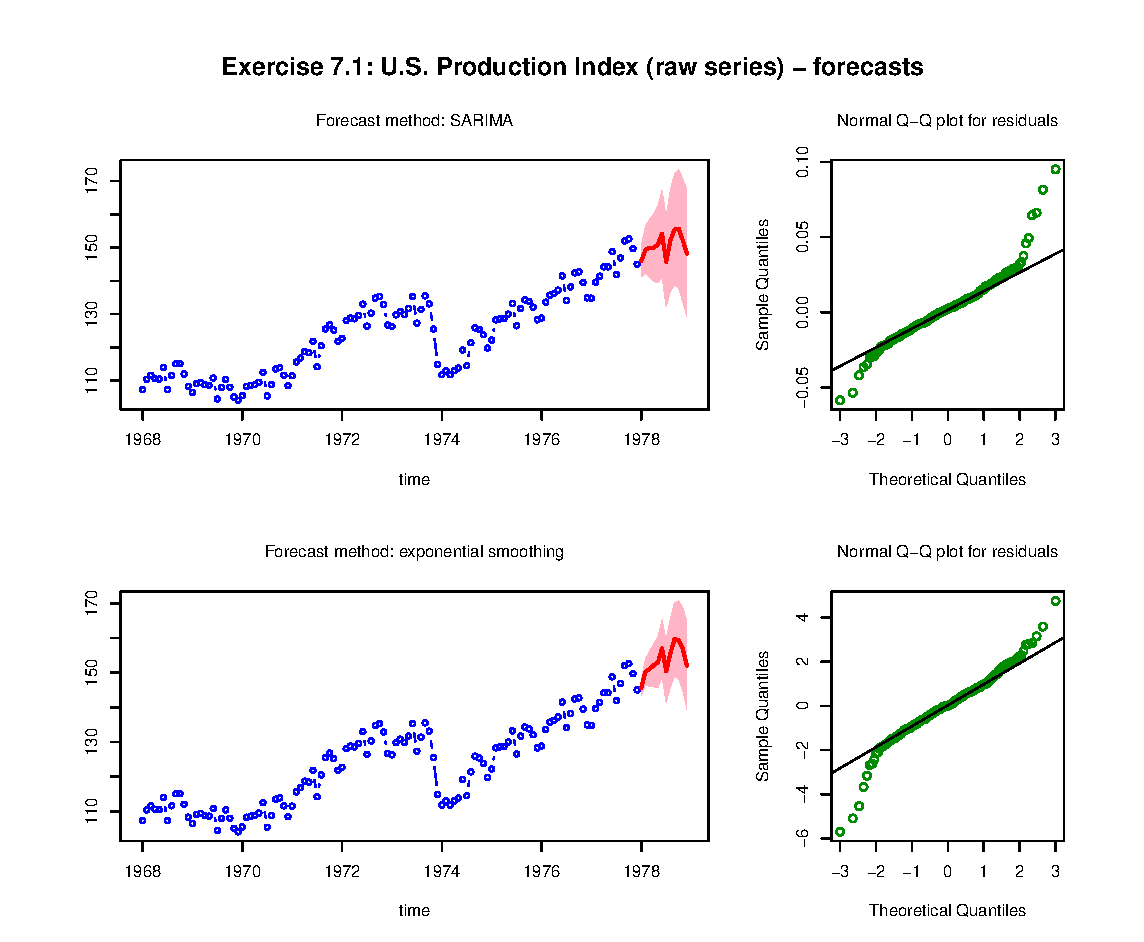
\includegraphics[width=0.8\textwidth]{plots/UsProdRawForecast.pdf}
\caption{U.S. Production Index Raw Forecasts}
\end{figure}

\begin{figure}[H]
\centering
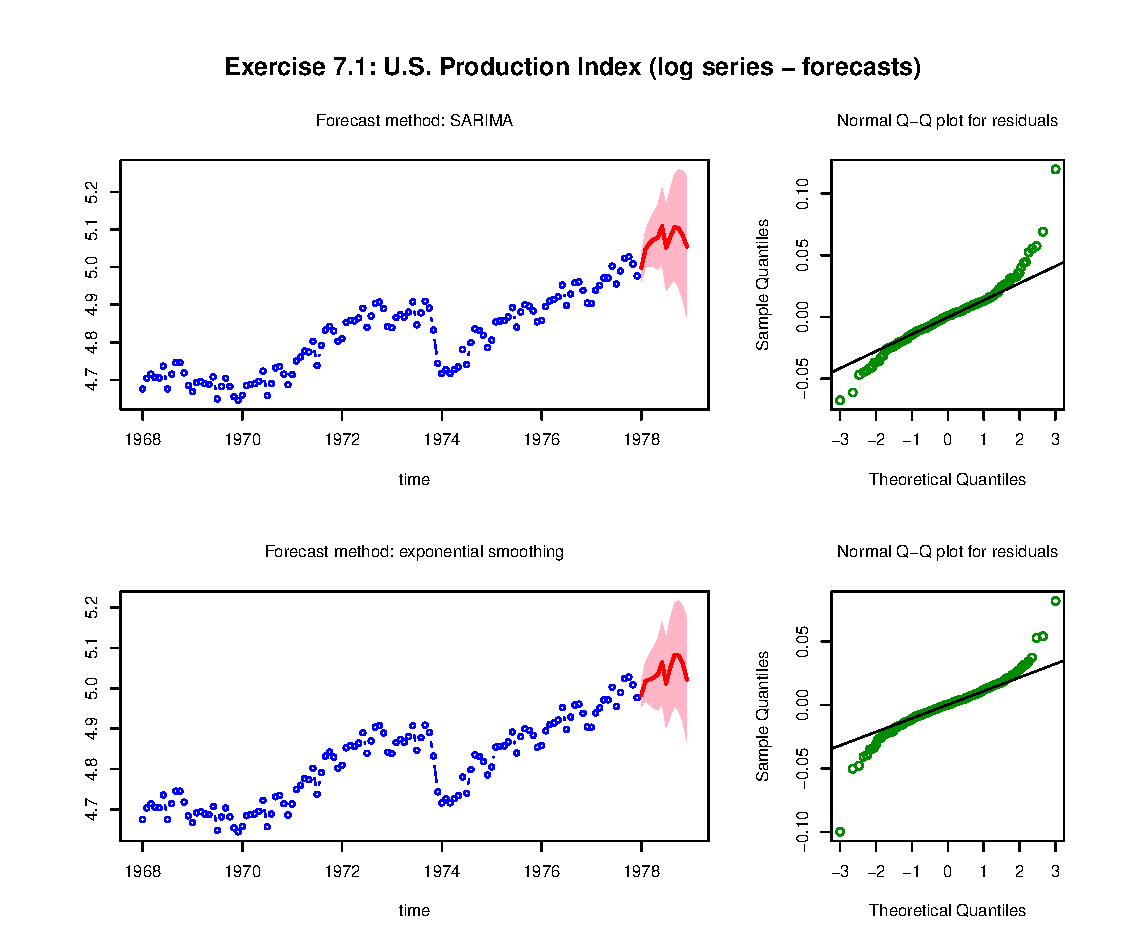
\includegraphics[width=0.8\textwidth]{plots/UsProdLogForecast.pdf}
\caption{U.S. Production Index Log Forecasts}
\end{figure}

The Q-Q Plots of the log series indicate that the residuals are closer to normality, while they still have some deviations at the tails. This suggests that the models on the log series capture the underlying pattern more effectively.